
%(BEGIN_QUESTION)
% Copyright 2010, Tony R. Kuphaldt, released under the Creative Commons Attribution License (v 1.0)
% This means you may do almost anything with this work of mine, so long as you give me proper credit

Sketch the necessary wire connections such that the lamp will turn {\it on} when the pushbutton switch is pressed and turn {\it off} when the pushbutton switch is released.  Assume that the pushbutton switch has {\it normally-open} (NO) contacts.  Ensure that the relay coil is powered by its own battery and the lamp by its own battery, with no connections between the two power sources:

$$\includegraphics[width=15.5cm]{i04763x01.eps}$$

\underbar{file i04763}
%(END_QUESTION)





%(BEGIN_ANSWER)

$$\includegraphics[width=15.5cm]{i04763x02.eps}$$

An alternative solution uses the NO contacts on the other side of the ice-cube relay.

%(END_ANSWER)





%(BEGIN_NOTES)

{\bf This question is intended for exams only and not worksheets!}.

%(END_NOTES)


